\section{Проект EXPERT}
Сейчас в мире существует несколько установок, позволяющих получать пучки экзотических ядер. В связи с актуальностью проблемы, ведется строительство и переоборудование уже существующих исследовательских комплексов: Facility for Rare Isotope Beams (FRIB) в NSCL MSU США, Facility for Antiproton and Ion Research (FAIR) в Институте Тяжелых Ионов (GSI) Германия, Radioactive Ion Beam Factory в RIKEN Япония, SPIRAL-2 в GANIL Франция, ACCULINNA-2 в ЛЯР ОИЯИ Россия. 
 

%Эксперименты на сепараторе АКУЛИНА были начаты в 1996г. На данный момент одной из самых перспективных идей является исследование экзотических ядер вблизи границы стабильности и за её пределами на установках АКУЛИНА и АКУЛИНА2. Масс-сепаратор АКУЛИНА на пучке циклотрона У-400М дает хорошие возможности для получения вторичных пучков высокого качества. Радиоактивные пучки получаются в результате первичного ускорения на циклотроне У-400М ионов 7Li, 11B, 13C, 15N, 18O. Основным преимуществом комплекса является высокая интенсивность первичного пучка, которая в непрерывном режиме облучения поддерживается на уровне $2.4\cdot10^{11}$ c$^{-1}$\cite{ufn}. Ионно-оптическая схема масс-сепаратора АКУЛИНА, а также ряд вспомогательных средств диагностики вторичных пучков позволяют фокусировать вторичные пучки на мишень площадью 0.8 см$^2$. Энергетический разброс пучков вторичных частиц составляет $\approx 5\%$\cite{ufn}. 
%Дополнительное измерение времени пролета ионов дает возможность повысить точность измерения энергии детектируемых ионов до 1\%.

%\begin{figure}[h]
%	\center{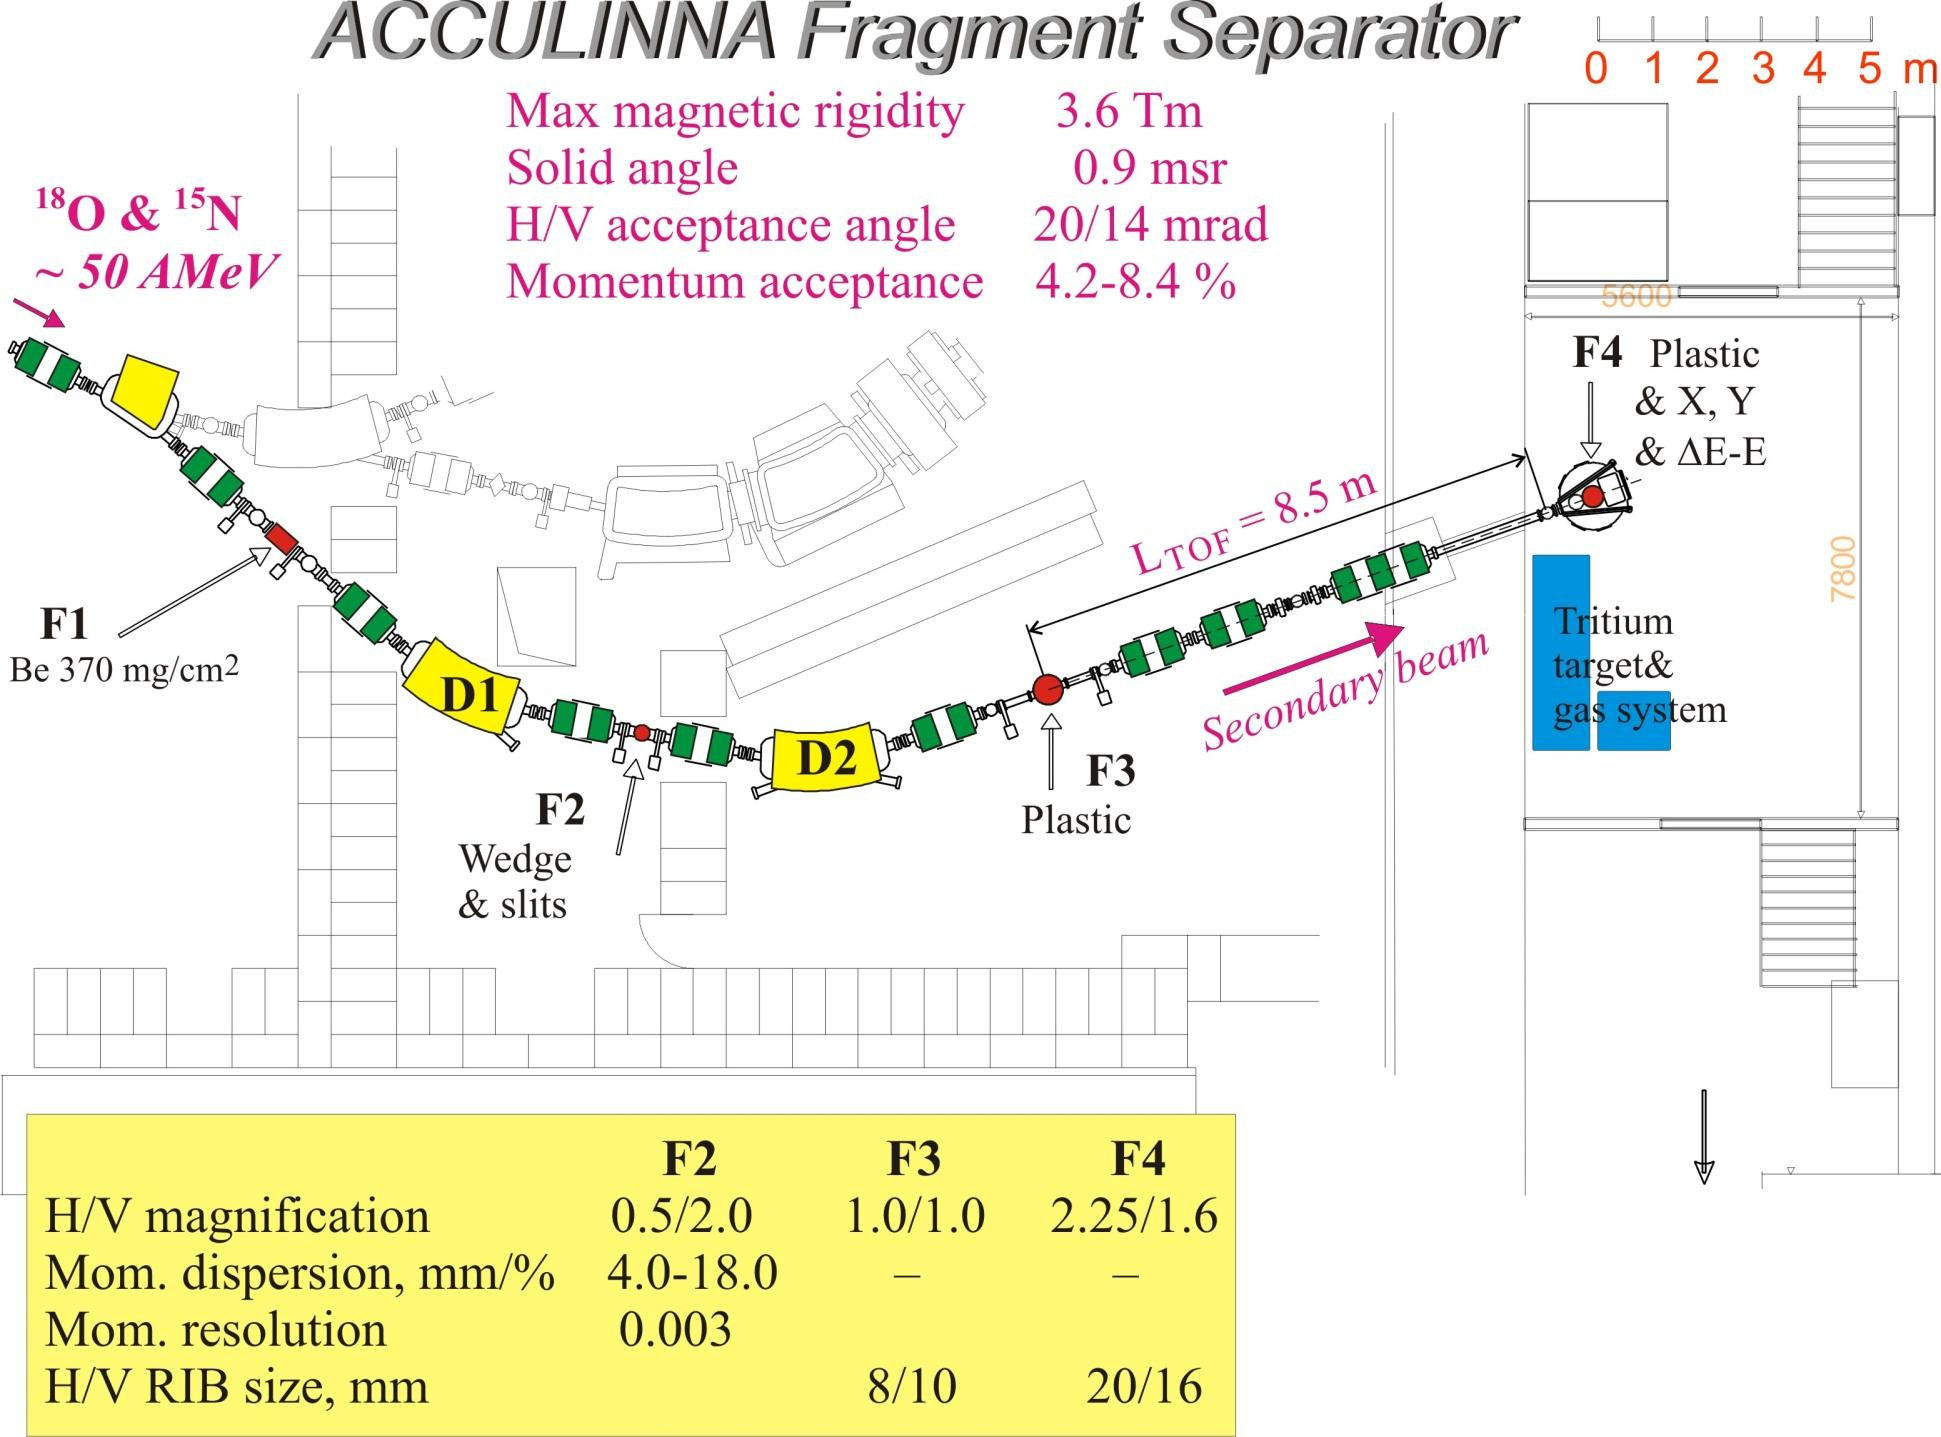
\includegraphics[width=1\linewidth]{aculina.png}}
%	\caption{Cепаратора АКУЛИНА. F1 - плоскость производящей мишени; F2 - плоскость промежуточной дисперсии; F3 - ахроматическая фокальная плоскость;F4 - вторая фокальная плоскость, D1 и D2 - магниты.}
%	\label{ris:aculina}
%\end{figure} 

Одной из установок ускорительного комплекса FAIR на базе Института Тяжелых Ионов в г. Дармштадт, Германия будет фрагмент-сепаратор Super-FRS (рис.~\ref{ris:FRS}). Super-FRS - сверхпроводящий фрагмент-сепаратор, служащий для получения пучков радиоактивных ядер методом in-flight. Super-FRS будет способен работать с пучками экзотических ядер вплоть до релятивистских энергий. Идентификация ионов будет проводиться методом измерения удельных потерь энергии  и времени пролета(Time of Flight). 

% \begin{figure}[h]
% 	\center{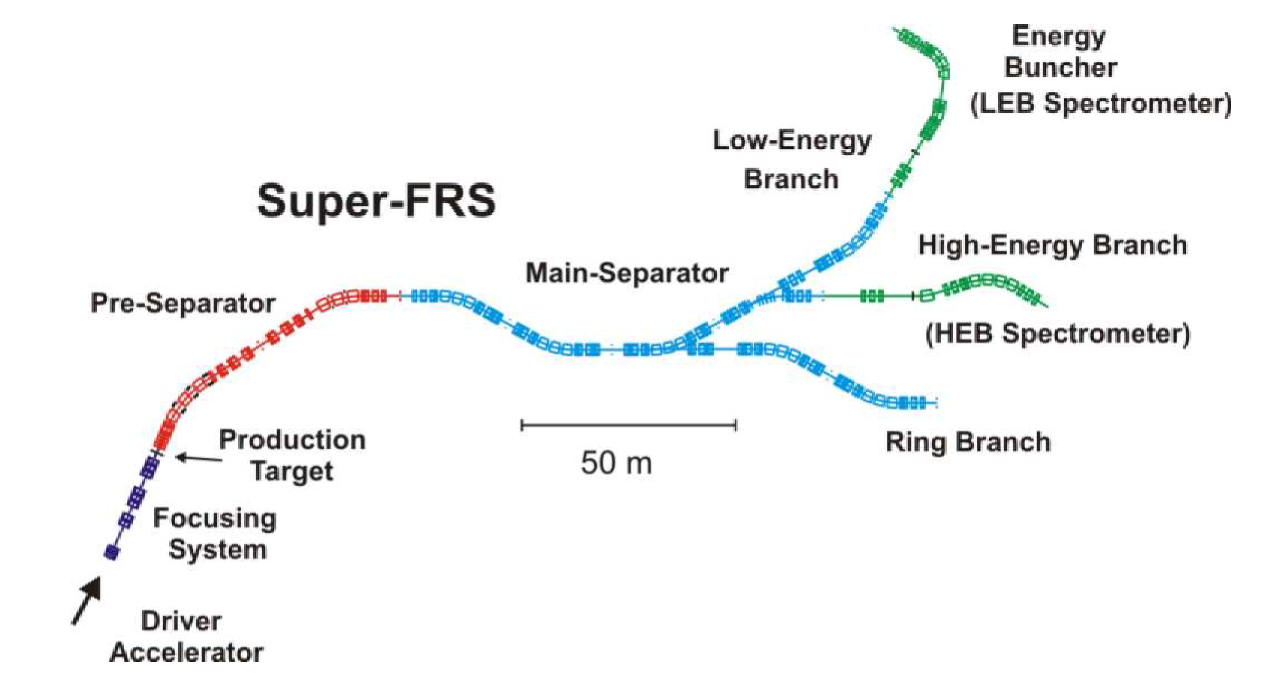
\includegraphics[width=1\linewidth]{FRS.png}}
% 	\caption{Схематическое изображение сверхпроводящего фрагмент-сепаратора Super-FRS. Системы идентификации частиц находятся на стадиях Pre-Separator и Main-Separator. Пучки редких изотопов доставляются в экспериментальные залы тремя ответвлениями от основного сепаратора: Ring Branch, High-Energy Branch и Energy Buncher [1].}
% 	\label{ris:FRS}
% \end{figure}

{
	\centering
	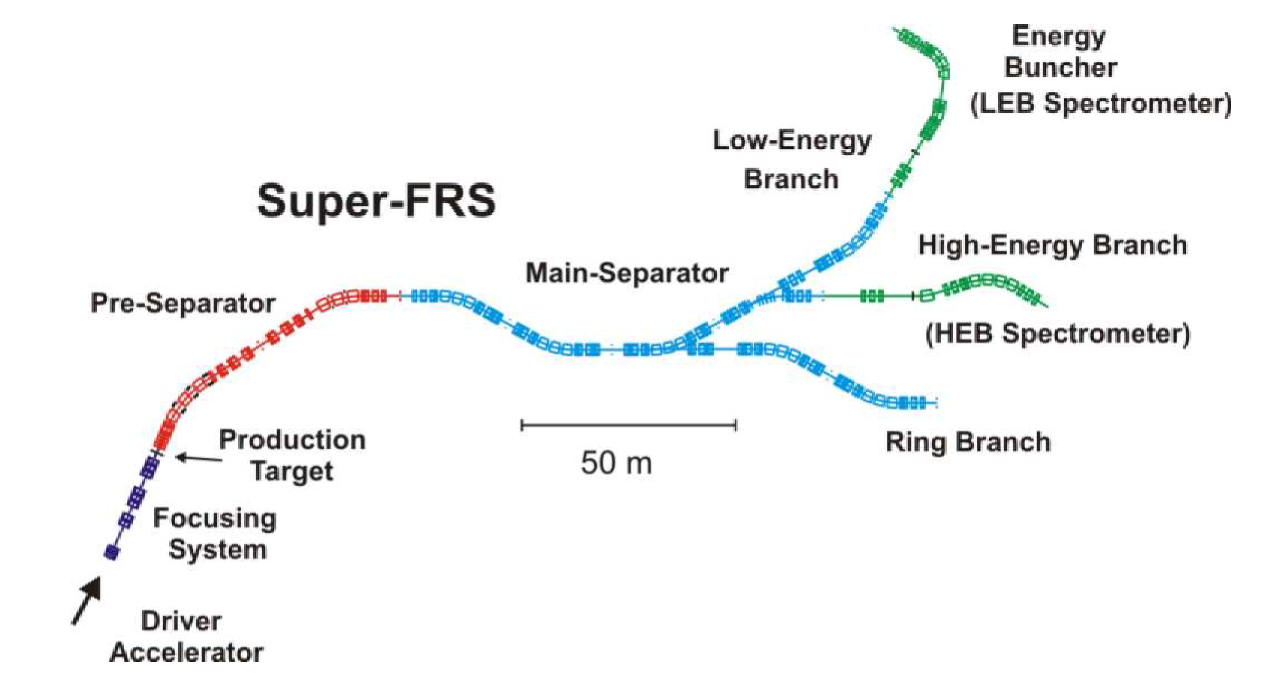
\includegraphics[width=1\linewidth]{FRS.png}
	\captionof{figure}{Схематическое изображение сверхпроводящего фрагмент-сепаратора Super-FRS. Системы идентификации частиц находятся на стадиях Pre-Separator и Main-Separator. Пучки редких изотопов доставляются в экспериментальные залы тремя ответвлениями от основного сепаратора: Ring Branch, High-Energy Branch и Energy Buncher \cite{FAIR}.}\label{ris:FRS}
}


Методика подобных измерений состоит, как правило, в следующем: на оси пучка на некотором расстоянии друг от друга (времяпролетная база) ставятся два детектора: «старт» и «стоп». Такие детекторы должны быть достаточно тонкими, чтобы энергетические потери в детекторе составляли лишь малую долю полной энергии частиц пучка. Эти детекторы должны регистрировать как время прохождения частицы, так и потерю энергии частицы в материале детектора. Зная величину базы и время, за которое частица прошла между двумя детекторами, можно вычислить скорость этой частицы $\beta$. 

При движении частицы в однородном магнитном поле (дипольного магнита фрагмент-сепаратора) величина магнитной жёсткости ($\xi$) связана с величиной вектора магнитной индукции $B$ соотношением \ref{Mag}.

%\begin{equation}
%\label{Mag}
%B \rho =  \frac{pc}{Ze},
%\end{equation}
%
%где $\rho$ - радиус кривизны траектории движения частицы.

Для налетающих частиц с энергиями, меньше 1 ГэВ, бомбардирующих тонкий поглотитель потери энергии ($\bigtriangleup E$) в первом приближении  определяются как:

\begin{equation}
\label{Bloh}
\bigtriangleup E \sim \frac{Z^2}{\beta^2},
\end{equation}
где $\beta = \frac{\nu}{c}$ - скорость частицы.

%\red{Одновременное измерение потерь энергии и времени пролёта позволяет однозначно идентифицировать частицы (Рис.~\ref{ris:iden}).}

%\begin{figure}[h]
%	\center{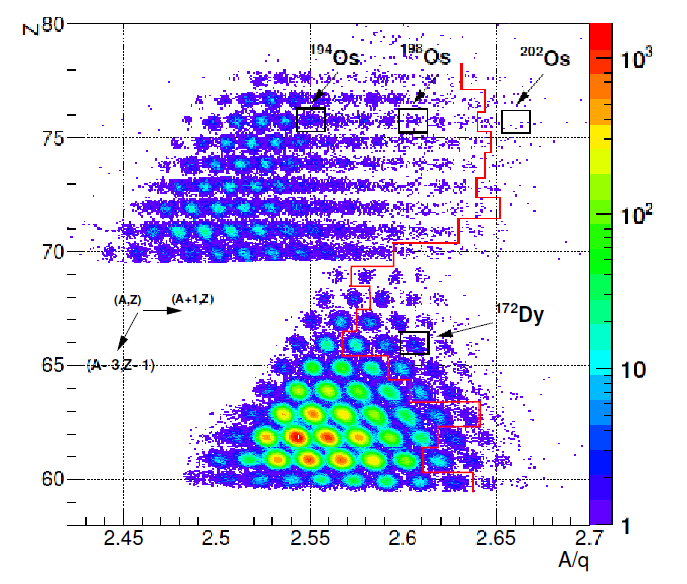
\includegraphics[width=1\linewidth]{identification.png}}
%	\caption{Пример идентификации изотопов ядер с Z $\sim$ 60 - 80 методом одновременного измерения потерь энергии и времени пролёта. Атомный номер Z и отношение массового числа к зарядовому состоянию $A/Q$ рассчитываются из величин магнитной жесткости $B\rho$, времени пролета и потерь энергии. Измерения проведены на In-Flight фрагмент-сепараторе FRS в GSI. Каждый пик на представленной двумерной гистограмме соответствует отдельному изотопу тяжелого элемента. Изображение взято из статьи [2]}
%	\label{ris:iden}
%\end{figure}

{
	\centering
	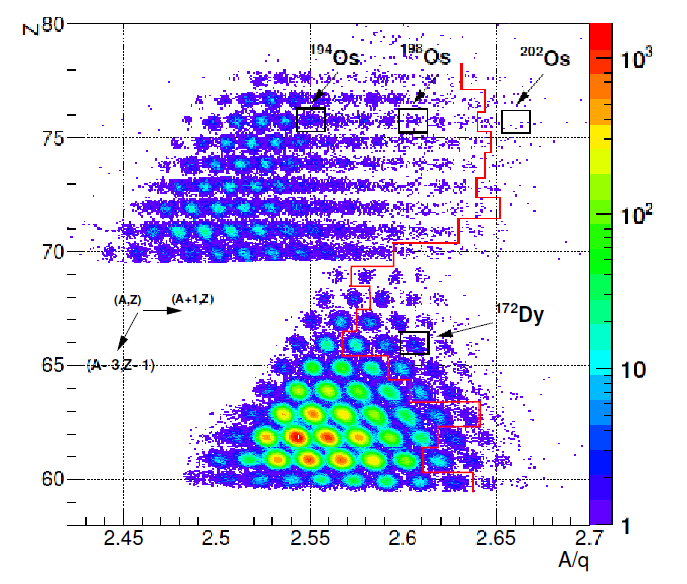
\includegraphics[width=1\linewidth]{identification.png}
	\captionof{figure}{Пример идентификации изотопов ядер с Z $\sim$ 60 - 80 методом одновременного измерения потерь энергии и времени пролёта. Атомный номер Z и отношение массового числа к зарядовому состоянию $A/Q$ рассчитываются из величин магнитной жесткости $B\rho$, времени пролета и потерь энергии. Измерения проведены на In-Flight фрагмент-сепараторе FRS в GSI. Каждый пик на представленной двумерной гистограмме соответствует отдельному изотопу тяжелого элемента. Изображение взято из статьи \cite{identificate}.}\label{ris:iden}
}

Надежность идентификации частицы и определение её энергии напрямую зависят от точности измерения момента времени прохождения частицы через соответствующий детектор, что, в свою очередь, определяется свойствами детектора.

\subsection{Проект EXPERT}
Проект EXPERT (EXotic Particle Emission and Radioactivity by Tracking) является частью программы Super-FRS Experiment. EXPERT представляет собой компактную модульную установку для проведения исследований чрезвычайно экзотических нестабильных ядер. 

%\begin{figure}[h]
%	\center{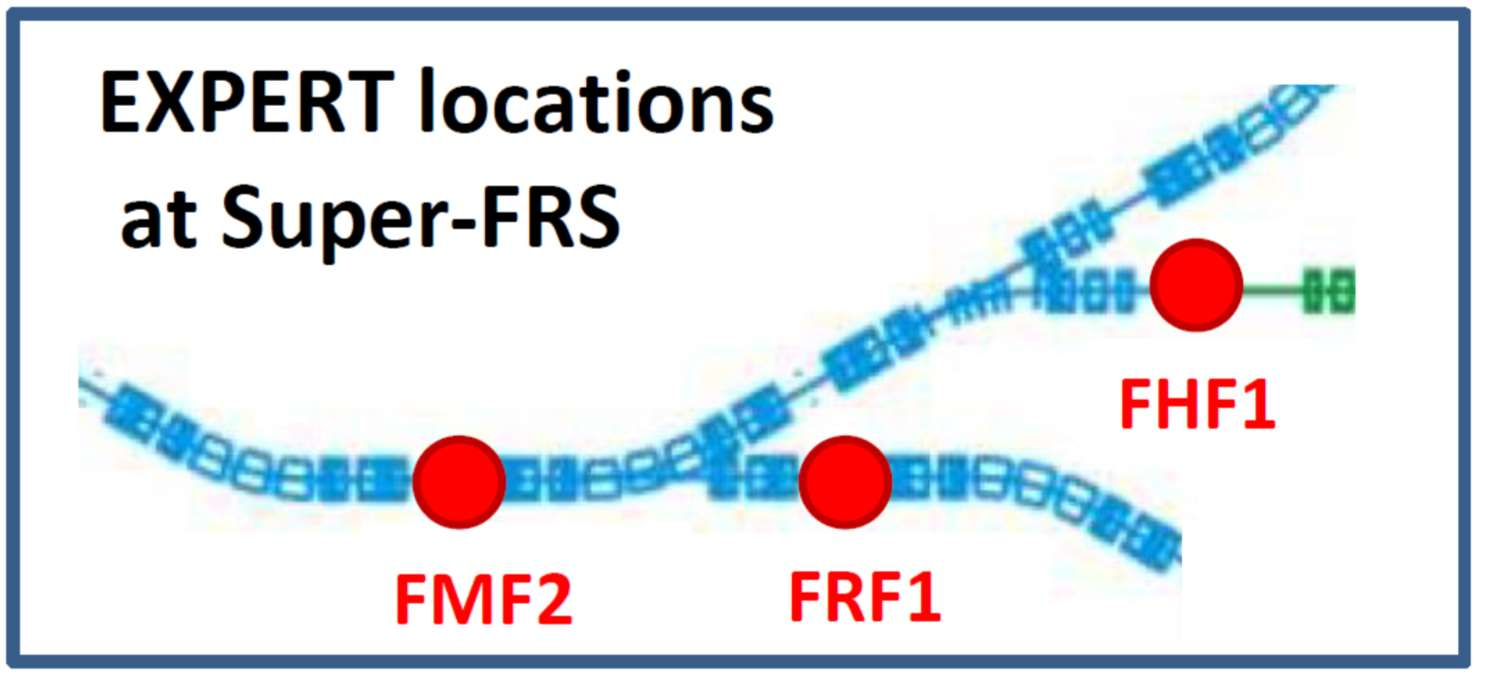
\includegraphics[width=1\linewidth]{frsexpert.png}}
%	\caption{Красными точками обозначено расположение детекторов EXPERT в экспериментах на сепараторе фрагментов Super-FRS.}
%	\label{ris:frsexpert}
%\end{figure}

{
	\centering
	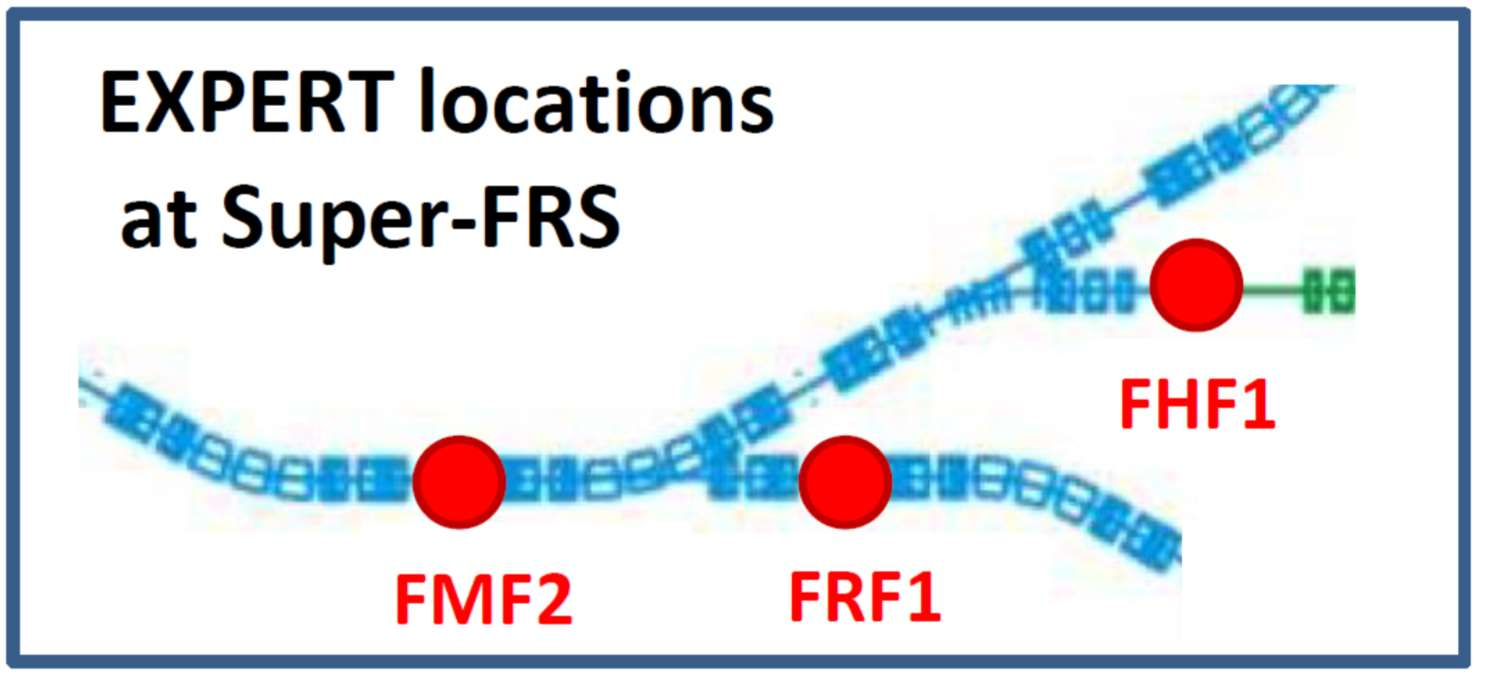
\includegraphics[width=1\linewidth]{frsexpert.png}
	\captionof{figure}{Красными точками обозначено расположение детекторов EXPERT в экспериментах на сепараторе фрагментов Super-FRS.}\label{ris:frsexpert}
}

Нестабильные ядра, находящиеся за пределами линий стабильности, либо распадаются в полете, либо испускают нуклоны, так как являются радиоактивными. Основными каналами распада таких ядер является испускание одного, двух или четырёх протонов или нейтронов. Продукты распада измеряются с помощью нескольких детектирующих модулей установки EXPERT. Установка схематически изображена на Рис.~\ref{ris:expert}. Её элементами  являются:


\begin{enumerate}
	\item Радиационно устойчивый кремниевый стриповый детектор (SSD), предоставляющий информацию о времени пролета, местоположении и потерях энергии ионов, и он будет использоваться для отслеживания вторичного луча, падающего на вторичную мишень.
	\item Детектор заряженных частиц состоящий из трёх слоев микростриповых кремниевых детекторов, позволяющий определять траектории всех продуктов распада экзотических ядер ($\mu$Si tracking).
	\item Детектор нейтронов с высоким угловым разрешением NeuRad (Neutron Radioactivity). При помощи NeuRad и микростриповых детекторов мы можем получать точную информацию об угловых корреляциях нейтронов распада и оставшегося заряженного фрагмента. С помощью этих данных, можно оценивать энергию распада экзотического ядра. Координаты тяжелого заряженного фрагмента могут быть получены из массива микростриповых кремниевых детекторов, а траектории нейтронов планируется получить с помощью детектора NeuRad. 
	\item Детектор гамма квантов GADAST (Gamma-ray Detectors Around Secondary Target). GADAST представляет собой  массив сцинтилляционных детекторов, измеряющий гамма-излучение и легкие заряженные частицы, испускаемые мгновенно после вторичной реакции. В
	эксперименте это позволит различить каналы распадов для тяжелых фрагментов с возбужденных состояний и мгновенного распада с возбуждённых состояний с испусканием гамма-излучения.
	\item Время-проекционная оптическая камера (OTPC) - устройство для 3D-реконструкции имплантированных многочастичных распадов ионов в конечной фокальной плоскости Super-FRS. Детектор позволяет оценить траектории всех заряженных фрагментов распада с временем жизни от 100 нс до 1 с. \cite{Super-FRS}
\end{enumerate}

Комбинируя вышеописанные модули для разных сценариев эксперимента могут быть изучены следующие явления:

\begin{itemize}
	\item Поиск и изучение структуры ядерных систем, расположенных далеко за пределами границы стабильности.
	\item Изучение экзотической двух-протонной, 2p, радиоактивности и поиск новых типов радиоактивных распадов: 4p, 2n, 4n.
	\item Исследования резонансных распадов p, 2p, 4p, 6p, n, 2n, 4n, 6n.
	\item Исследования запаздывающего бета распада экзотических изотопов.
\end{itemize}

%\begin{figure}[h]
%	\center{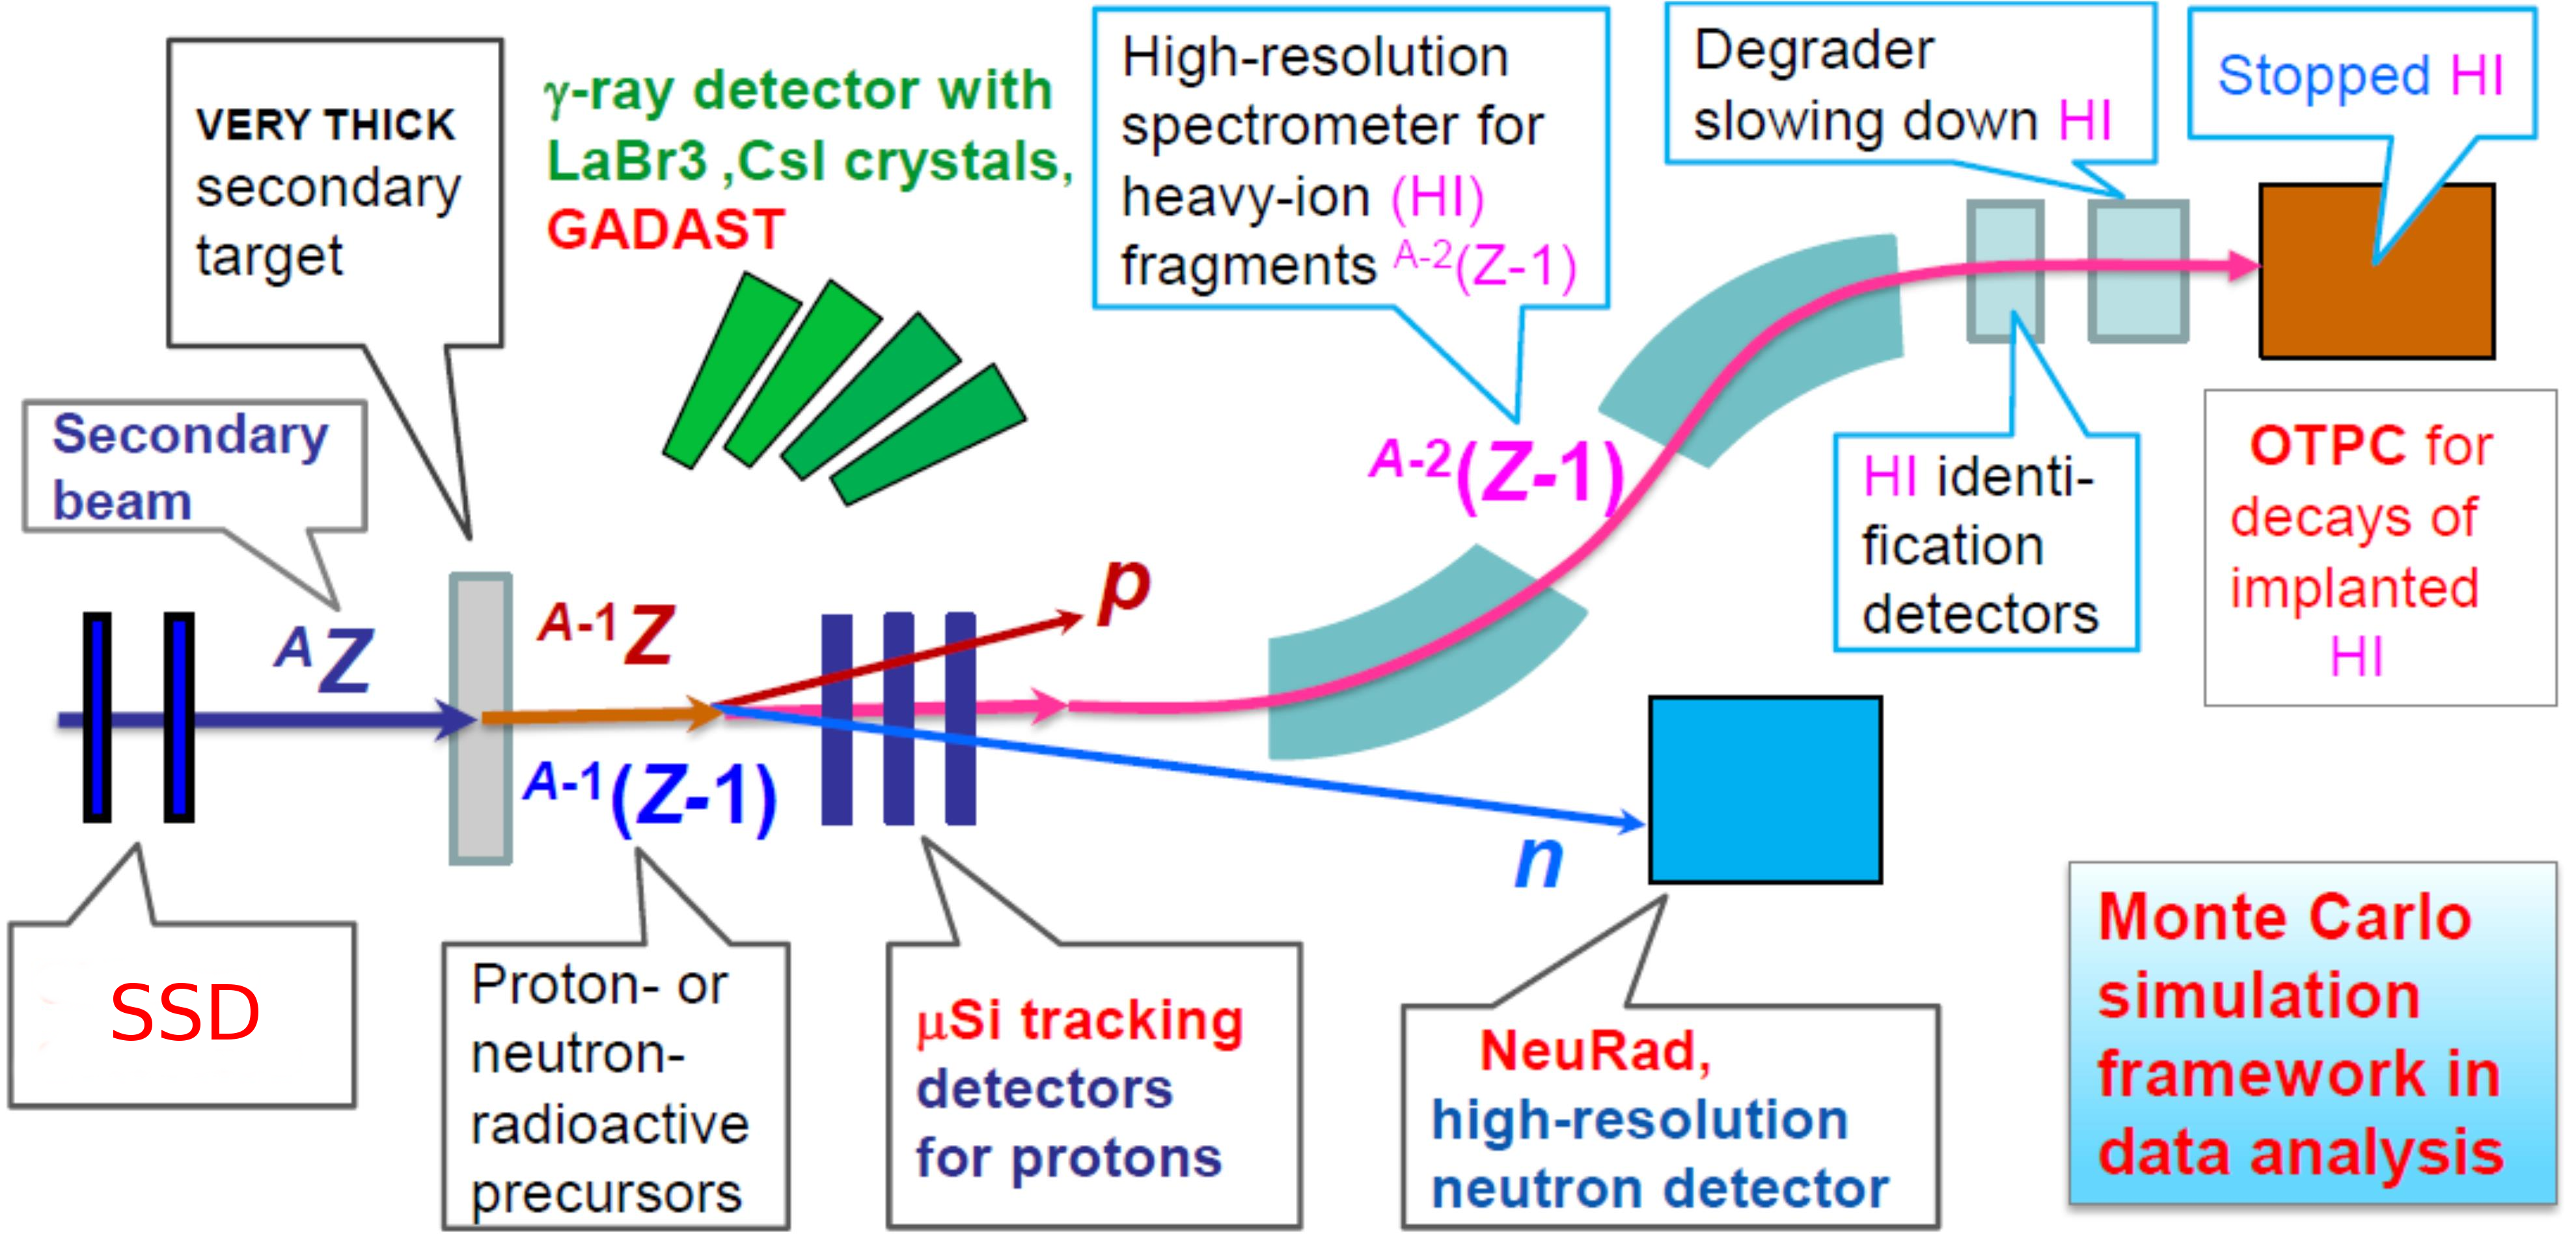
\includegraphics[width=1\linewidth]{expert.png}}
%	\caption{Схематическое изображение предлагаемых экспериментов нестабильных ядер за пределами протонной и нейтронной стабильности.}
%	\label{ris:expert}
%\end{figure}
{
	\centering
	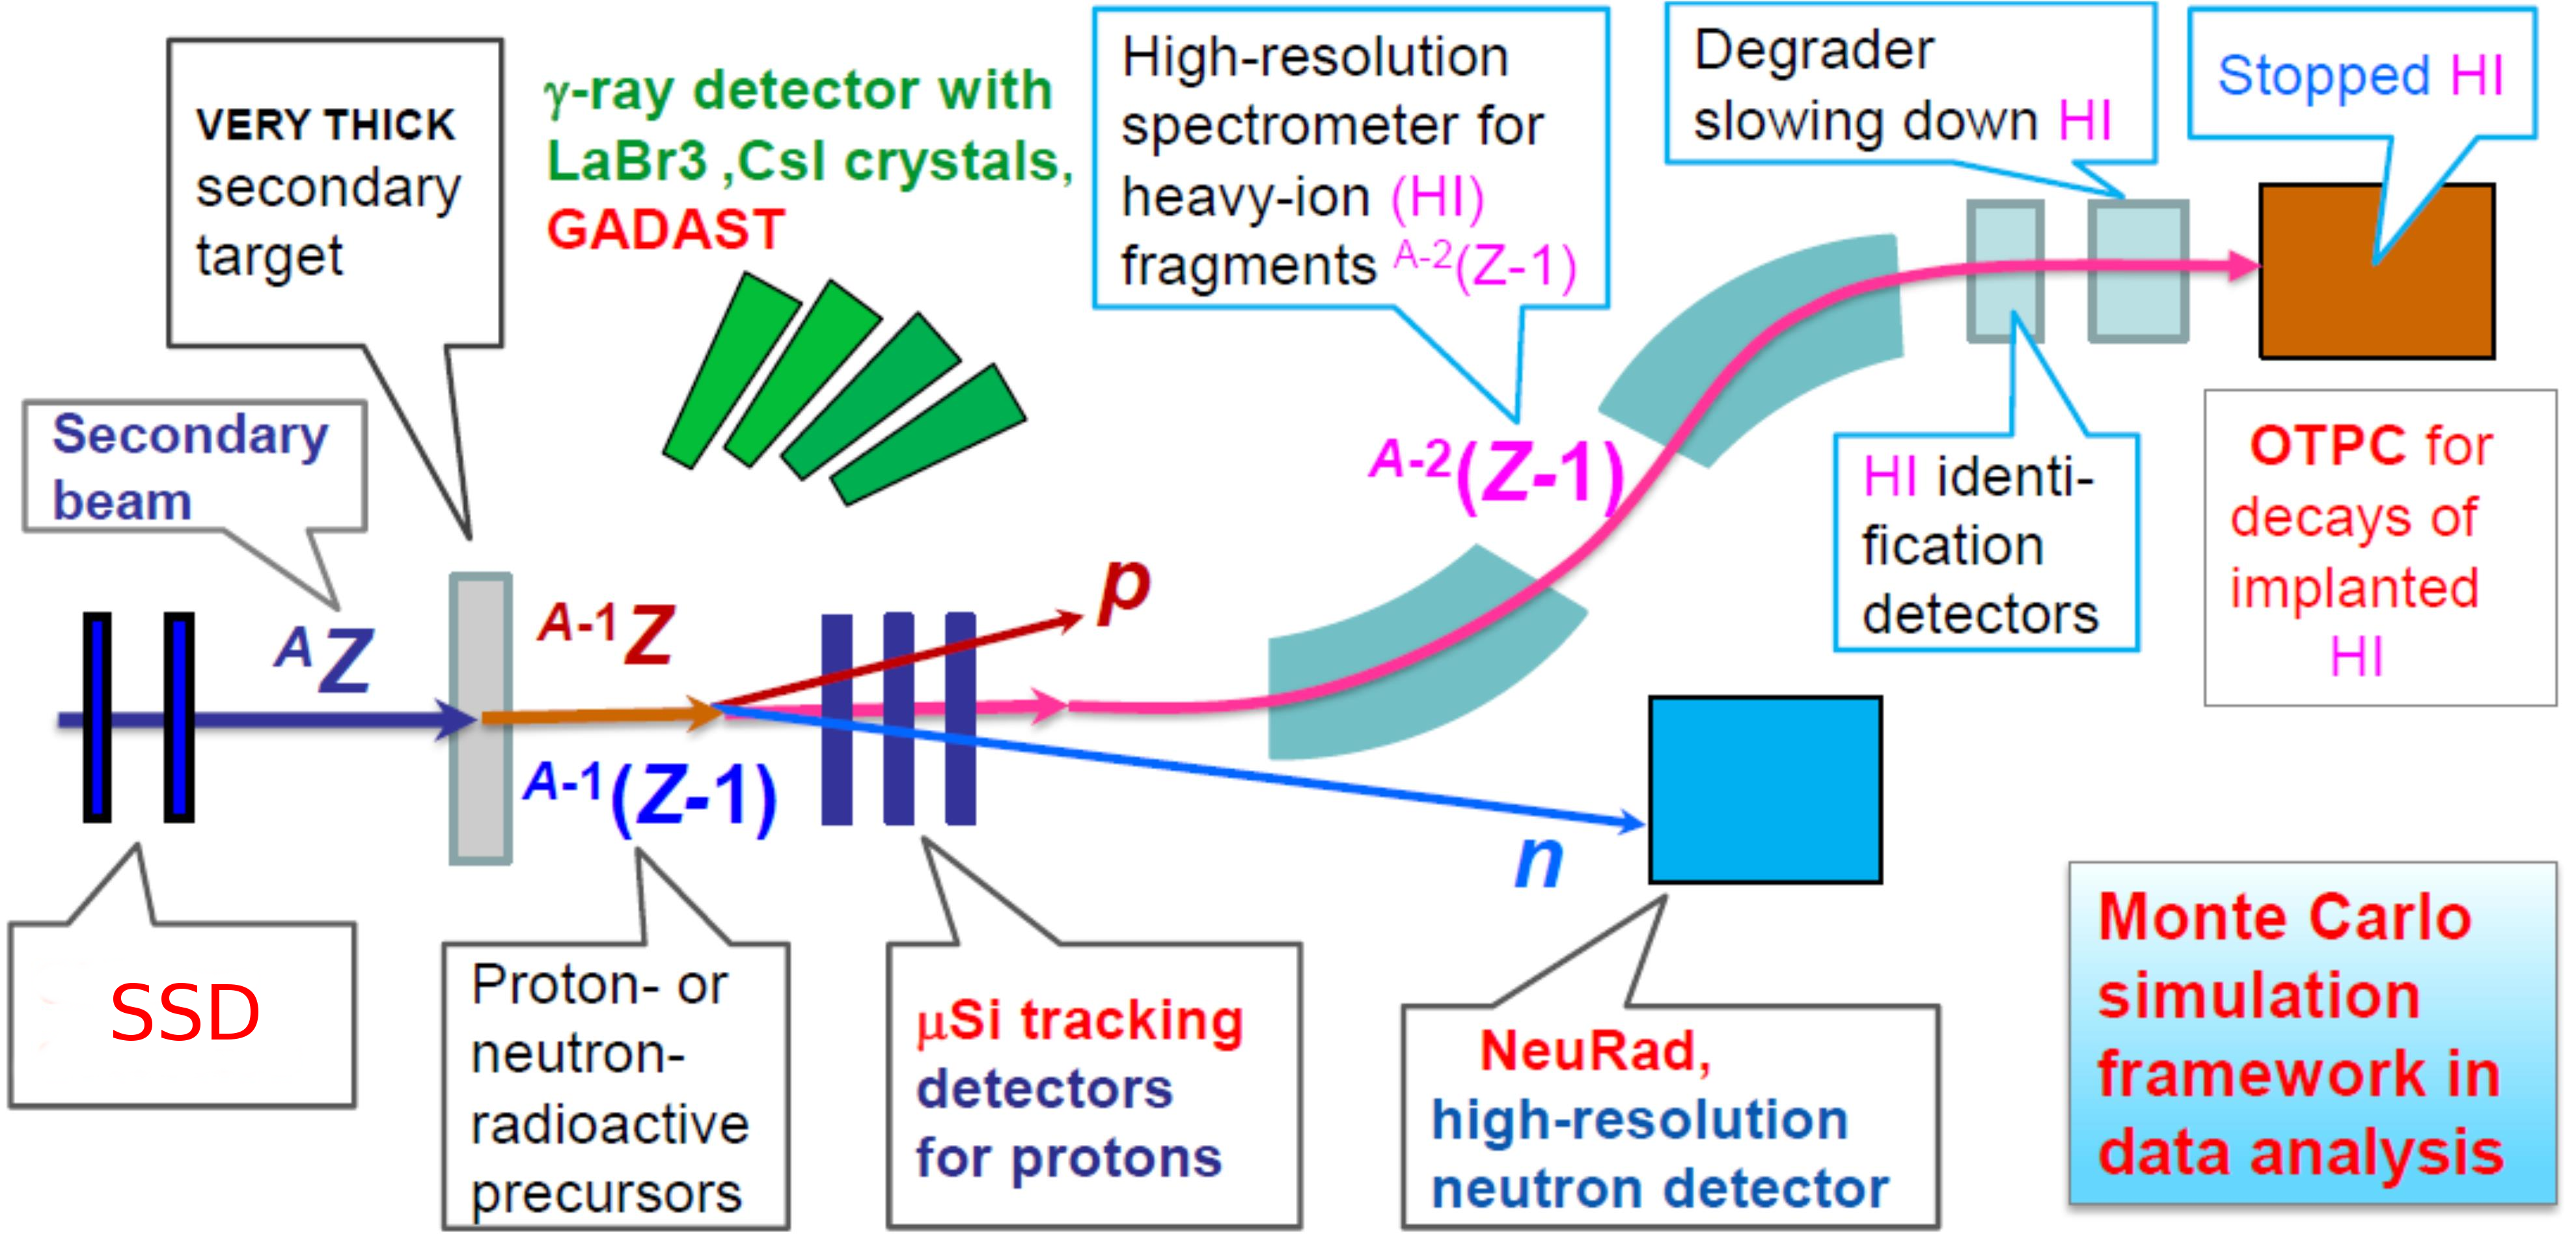
\includegraphics[width=1\linewidth]{expert.png}
	\captionof{figure}{Схематическое изображение предлагаемых экспериментов нестабильных ядер за пределами протонной и нейтронной стабильности\cite{Super-FRS}. Описание выше.}\label{ris:expert}
}


\subsection{Детектор NeuRad}
Разрабатываемый детектор нейтронов NeuRad предназначен для получения прецизионной информации об угловых корреляциях нейтронов распада с заряженным фрагментом. Эта информация используется для определения энергии распада, происходящего вблизи мишени, и времени жизни экзотического ядра. Информация о направлении вылета тяжелого фрагмента поступает от кремниевого микрострипового детектора, а направления полёта нейтронов должны быть получены с помощью детектора NeuRad. 

Детектор NeuRad будет состоять из большого количества оптических волокон ($\approx$ 10000 штук) изготовленных из пластмассового сцинтиллятора BCF12 (см. Таблица \ref{tab:bolts}). Каждое волокно имеет квадратное сечение $3\times3$ мм$^2$ и длину 1 м. На поверхность волокон нанесён тонкий слой акрила и несколько слоёв специальной светоизолирующей краски для уменьшения вероятности прохождения света из одного волокна в другое. Сцинтиллирующие волокна собраны в пучки.

{
	\centering
	\begin{tabular}{|c|c|}
		\hline
		Материал пластика: & Полистирол \\
		\hline
		Показатель преломления полистирола: & \textbf{1.6}  \\
		\hline
		Плотность полистирола [г/см$^3$]: & \textbf{1.05} \\
		\hline
		Изолирующий материал покрытия: & Акрил \\
		\hline
		Толщина покрытия: & \textbf{4\%} от толщины волокна  \\
		\hline
		Показатель преломления акрила: & \textbf{1.49} \\
		\hline
		Длина волны производимого света [нм]: & \textbf{435} \\
		\hline
		Время высвечивания [нс]: & \textbf{3.2} \\
		\hline
		Световыход, количество фотонов, & \\  
		порождаемых 1МэВ потерянной энергии: & \textbf{8000} \\
		\hline
	\end{tabular}
	\captionof{table}{ Свойства оптического волокна \cite{crystals}}\label{tab:bolts}
}

В экспериментах детектор будет установлен так, чтобы волокна были направлены вдоль траектории движения нейтронов (Рис.~\ref{ris:neuradPrinciple}). Такое расположение обеспечит более точную оценку положения взаимодействия нейтрона с детектором. 

Заряженная частица возбуждает молекулы сцинтиллятора, что приводит к появлению вспышки света.



%\begin{table}[H]
%\caption{\label{tab:bolts} Свойства материалов детектора\cite{crystals}}
%	\begin{center}
%		\begin{tabular}{|c|c|}
%			\hline
%			Материал пластика: & Полистирол \\
%			\hline
%			Показатель преломления полистирола: & \textbf{1.6}  \\
%			\hline
%			Плотность полистерола [г/см$^3$]: & \textbf{1.05} \\
%			\hline
%			Изолирующий материал покрытия: & Акрил \\
%			\hline
%			Толщина покрытия: & \textbf{4\%} от толщины волокна  \\
%			\hline
%			Показатель преломления акрила: & \textbf{1.49} \\
%			\hline
%			Длина волны производимого света[нм]: & \textbf{435} \\
%			\hline
%			Время высвечивания[нс]: & \textbf{3.2} \\
%			\hline
%			Световыход, количество фотонов, & \\  
%			порождаемых 1МэВ потерянной энергии: & \textbf{8000} \\
%			\hline
%		\end{tabular}
%	\end{center}
%\end{table}


%\begin{figure}[!ht]
%	\centering
%	\begin{tabular}{cc}
%		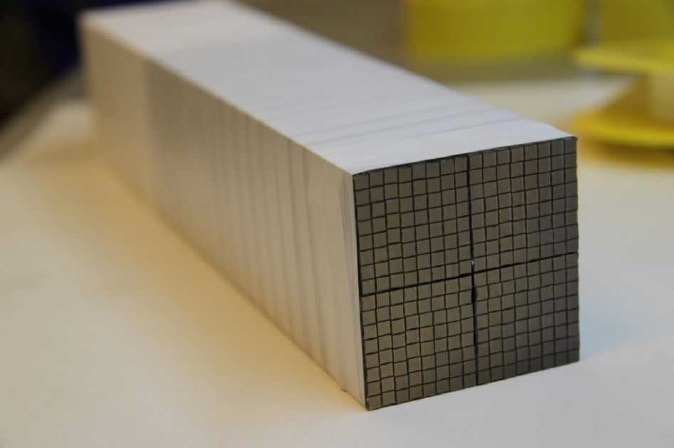
\includegraphics[width=0.5\linewidth]{neuradfibers.png} & 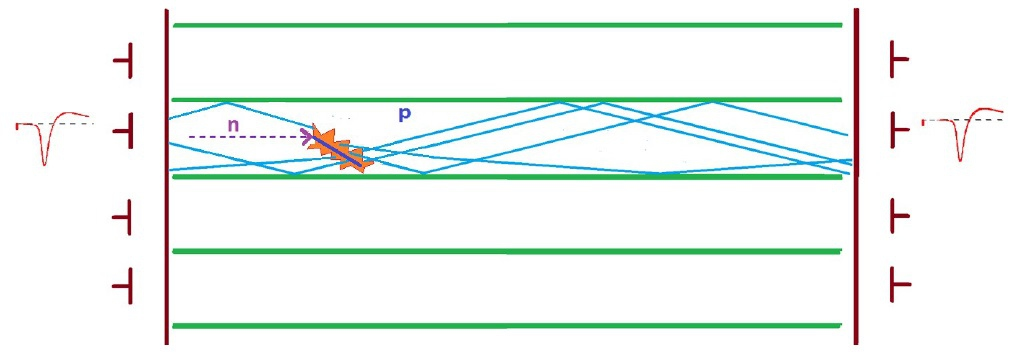
\includegraphics[width=0.5\linewidth]{neurad.png} \\
%		a) & b) \\
%	\end{tabular}
%	%	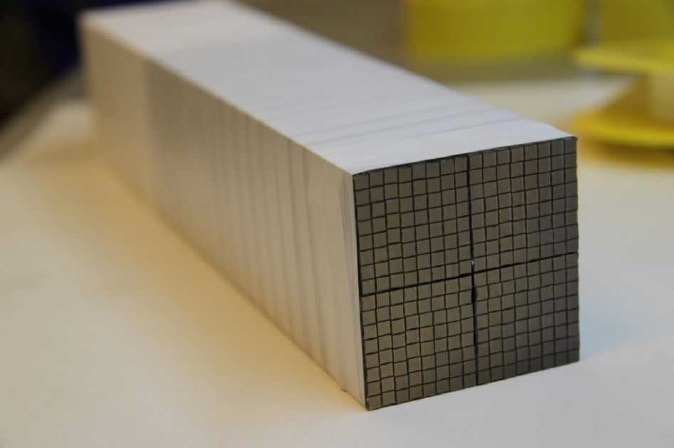
\includegraphics[width=1\linewidth]{neuradfibers.png}
%	\caption{Тестовый прототип NeuRad'a длиной 25 см, состоящий из 256 оптических волокон.}
%	\label{ris:neuradfibers}
%\end{figure}

%\begin{figure}[h]
%	\center{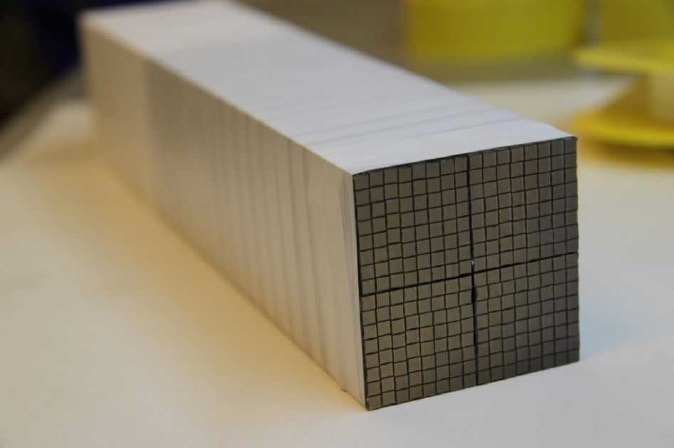
\includegraphics[width=1\linewidth]{neuradfibers.png}}
%	\caption{Тестовый прототип NeuRad'a длиной 25 см, состоящий из 256 оптических волокон.}
%	\label{ris:neuradfibers}
%\end{figure}

Нейтрон – частица, не имеющая заряда и не способная ионизировать вещество. Поэтому нейтрон регистрируют косвенно. При попадании нейтрона в объём сцинтиллятора, происходит ядерная реакция выбивания заряженной частицы, в большинстве случаев протона, называемого протоном отдачи. В таком случае, протон отдачи, получивший энергию от нейтрона, достаточно быстро её теряет, возбуждая молекулы сцинтиллятора. Излучённый свет сцинтиллятора перемещается до границ детектора, где расположены ФЭУ, из сигналов которых можно определить время прихода сигналов с двух сторон волокна. 

\begin{figure}[h]
	\center{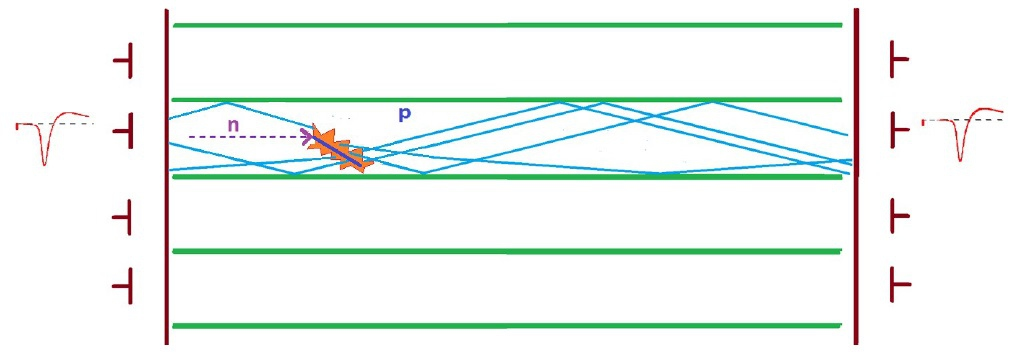
\includegraphics[width=1\linewidth]{neurad.png}}
	\caption{Принцип действия NeuRad.}
	\label{ris:neuradPrinciple}
\end{figure}
%{
%	\centering
%	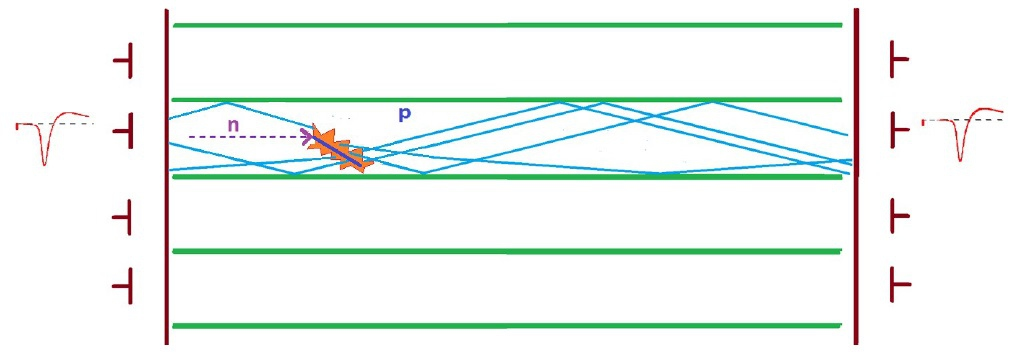
\includegraphics[width=1\linewidth]{neurad.png}
%	\captionof{figure}{Принцип действия NeuRad.}\label{ris:neuradPrinciple}
%}

Таким образом, каждому событию соответствуют времена сигналов с двух сторон оптического волокна $\tau_1$ и $\tau_2$. 
Разность величин $\Delta \tau = \tau_1 - \tau_2$ говорит о том, насколько быстрее пришёл сигнал с одной стороны, чем с другой. 
Так как, детектирующие устройства с обоих сторон одинаковы, то ненулевую разницу времён сигналов можно объяснить только тем, что фотонам, испущенные сцинтиллятором, потребовалось разное количество времени, чтобы достичь ФЭУ. То есть, величина $\Delta\tau$ соответствует определённой продольной координате взаимодействия налетающей частицы с материалом детектора. Исходя из этого, можно определять продольную координату взаимодействия по формуле
\begin{equation}
\label{koordinate}
\vec{Z} = \Delta \tau \frac{c}{n},
\end{equation}
где $\vec{Z}$ - вектор положения взаимодействия; ноль соответствует середине оптического волокна, n - абсолютный показатель материала волокна.

Одной из важных характеристик NeuRad, которая заслуживает особого внимания, является временное разрешение.  Уравнение 
\begin{equation} \label{eq:distance}
\delta(\Delta \tau) = \frac{n\cdot\delta Z}{c},
\end{equation}
где n - абсолютный показатель среды, с - скорость света, $\delta(\Delta \tau)$ и $\delta$Z - неопределённость по времени и координате соответственно, показывает, что для того, чтобы получить разрешение по продольной координате 10\,см, необходимо иметь неопределенность во времени меньше, чем 0,55\,нс. 

Временное разрешение также важно для того, чтобы отличать момент первого попадания нейтрона. Эта информация одновременно необходима для различия много-нейтронного события от множественного попадания одного и того же повторно рассеянного нейтрона и для проверки правдоподобия данных.